\documentclass[11pt]{amsart}

\usepackage{amsmath,amsthm}
\usepackage{amssymb}
\usepackage{graphicx}
\usepackage{enumerate}
\usepackage{fullpage}
% \usepackage{euscript}
% \makeatletter
% \nopagenumbers
\usepackage{verbatim}
\usepackage{color}
\usepackage{hyperref}

\usepackage{fullpage,tikz,float}
%\usepackage{times} %, mathtime}

\textheight=600pt %574pt
\textwidth=480pt %432pt
\oddsidemargin=15pt %18.88pt
\evensidemargin=18.88pt
\topmargin=10pt %14.21pt

\parskip=1pt %2pt

% define theorem environments
\newtheorem{theorem}{Theorem}    %[section]
%\def\thetheorem{\unskip}
\newtheorem{proposition}[theorem]{Proposition}
%\def\theproposition{\unskip}
\newtheorem{conjecture}[theorem]{Conjecture}
\def\theconjecture{\unskip}
\newtheorem{corollary}[theorem]{Corollary}
\newtheorem{lemma}[theorem]{Lemma}
\newtheorem{sublemma}[theorem]{Sublemma}
\newtheorem{fact}[theorem]{Fact}
\newtheorem{observation}[theorem]{Observation}
%\def\thelemma{\unskip}
\theoremstyle{definition}
\newtheorem{definition}{Definition}
%\def\thedefinition{\unskip}
\newtheorem{notation}[definition]{Notation}
\newtheorem{remark}[definition]{Remark}
% \def\theremark{\unskip}
\newtheorem{question}[definition]{Question}
\newtheorem{questions}[definition]{Questions}
%\def\thequestion{\unskip}
\newtheorem{example}[definition]{Example}
%\def\theexample{\unskip}
\newtheorem{problem}[definition]{Problem}
\newtheorem{exercise}[definition]{Exercise}

\numberwithin{theorem}{section}
\numberwithin{definition}{section}
\numberwithin{equation}{section}

\def\reals{{\mathbb R}}
\def\torus{{\mathbb T}}
\def\integers{{\mathbb Z}}
\def\rationals{{\mathbb Q}}
\def\naturals{{\mathbb N}}
\def\complex{{\mathbb C}\/}
\def\distance{\operatorname{distance}\,}
\def\support{\operatorname{support}\,}
\def\dist{\operatorname{dist}\,}
\def\Span{\operatorname{span}\,}
\def\degree{\operatorname{degree}\,}
\def\kernel{\operatorname{kernel}\,}
\def\dim{\operatorname{dim}\,}
\def\codim{\operatorname{codim}}
\def\trace{\operatorname{trace\,}}
\def\dimension{\operatorname{dimension}\,}
\def\codimension{\operatorname{codimension}\,}
\def\nullspace{\scriptk}
\def\kernel{\operatorname{Ker}}
\def\p{\partial}
\def\Re{\operatorname{Re\,} }
\def\Im{\operatorname{Im\,} }
\def\ov{\overline}
\def\eps{\varepsilon}
\def\lt{L^2}
\def\curl{\operatorname{curl}}
\def\divergence{\operatorname{div}}
\newcommand{\norm}[1]{ \|  #1 \|}
\def\expect{\mathbb E}
\def\bull{$\bullet$\ }
\def\det{\operatorname{det}}
\def\Det{\operatorname{Det}}
\def\rank{\mathbf r}
\def\diameter{\operatorname{diameter}}

\def\t2{\tfrac12}

\newcommand{\abr}[1]{ \langle  #1 \rangle}

\def\newbull{\medskip\noindent $\bullet$\ }
\def\field{{\mathbb F}}
\def\cc{C_c}



% \renewcommand\forall{\ \forall\,}

% \newcommand{\Norm}[1]{ \left\|  #1 \right\| }
\newcommand{\Norm}[1]{ \Big\|  #1 \Big\| }
\newcommand{\set}[1]{ \left\{ #1 \right\} }
%\newcommand{\ifof}{\Leftrightarrow}
\def\one{{\mathbf 1}}
\newcommand{\modulo}[2]{[#1]_{#2}}

\def\bd{\operatorname{bd}\,}
\def\cl{\text{cl}}
\def\nobull{\noindent$\bullet$\ }

\def\scriptf{{\mathcal F}}
\def\scriptq{{\mathcal Q}}
\def\scriptg{{\mathcal G}}
\def\scriptm{{\mathcal M}}
\def\scriptb{{\mathcal B}}
\def\scriptc{{\mathcal C}}
\def\scriptt{{\mathcal T}}
\def\scripti{{\mathcal I}}
\def\scripte{{\mathcal E}}
\def\scriptv{{\mathcal V}}
\def\scriptw{{\mathcal W}}
\def\scriptu{{\mathcal U}}
\def\scriptS{{\mathcal S}}
\def\scripta{{\mathcal A}}
\def\scriptr{{\mathcal R}}
\def\scripto{{\mathcal O}}
\def\scripth{{\mathcal H}}
\def\scriptd{{\mathcal D}}
\def\scriptl{{\mathcal L}}
\def\scriptn{{\mathcal N}}
\def\scriptp{{\mathcal P}}
\def\scriptk{{\mathcal K}}
\def\scriptP{{\mathcal P}}
\def\scriptj{{\mathcal J}}
\def\scriptz{{\mathcal Z}}
\def\scripts{{\mathcal S}}
\def\scriptx{{\mathcal X}}
\def\scripty{{\mathcal Y}}
\def\frakv{{\mathfrak V}}
\def\frakG{{\mathfrak G}}
\def\aff{\operatorname{Aff}}
\def\frakB{{\mathfrak B}}
\def\frakC{{\mathfrak C}}

\def\symdif{\,\Delta\,}
\def\mustar{\mu^*}
\def\muplus{\mu^+}

\def\soln{\noindent {\bf Solution.}\ }


%\pagestyle{empty}
%\setlength{\parindent}{0pt}

\begin{document}

\begin{center}{\bf Math 202A --- UCB, Fall 2016 --- William Guss}
\\
{\bf Problem Set 10, due Wednesday November 2}
\begin{tikzpicture}
\foreach \i in {1,...,4}
{
	\draw (\i -7,0) rectangle (\i-7+0.5,0.5);
	\draw [->] (\i-7 +0.25  ,0.5) -- (-4.25 ,1);
}
\draw (-4.5,1) rectangle (-4,1.5);
\draw [->] (-4.25 ,1.5) -- (-4.25 ,2);
\node[text width=3cm] at (-2.85,-0.25) {$\scripts_1$};
\foreach \i in {1,...,4}
{
	\draw (\i -1,0) rectangle (\i-1+0.5,0.5);
}
\foreach \i in {1,...,3}
{
	\draw (\i-1 + 0.5 ,1) rectangle (\i-1+1,1.5);
	\draw [->] (\i-1 +0.25  ,0.5) -- (\i-1 + 0.75 ,1);
	\draw [->] (\i-1 +1.25  ,0.5) -- (\i-1 + 0.75 ,1);
	\draw [->] (\i-1 + 0.75 ,1.5) -- (1.75 ,2);
}
\draw (1.5 ,2) rectangle (2,2.5);
\draw [->] (1.75 ,2.5) -- (1.75 ,3);
\node[text width=3cm] at (3.15,-0.25) {$\scripts_2$};
\end{tikzpicture}
%
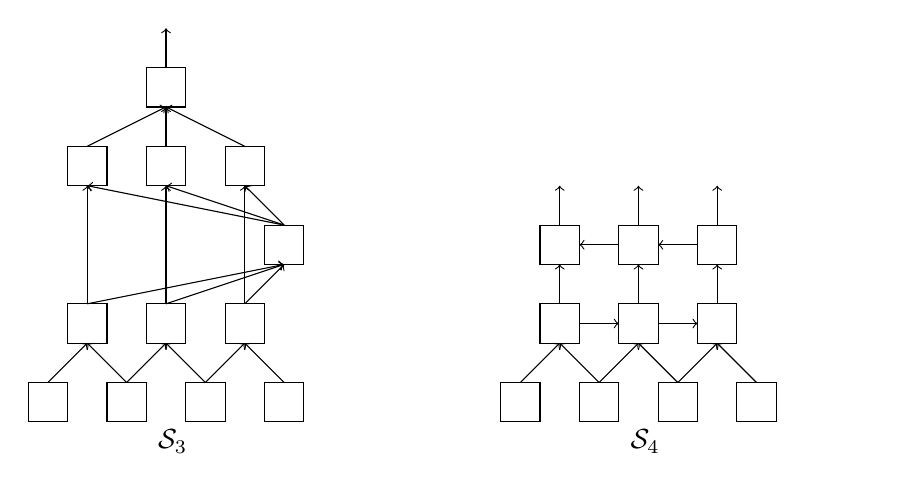
\begin{tikzpicture}
\foreach \i in {1,...,4}
{
	\draw (\i -7,0) rectangle (\i-7+0.5,0.5);
}
\foreach \i in {1,...,3}
{
	\draw (\i-7 + 0.5 ,1) rectangle (\i-7+1,1.5);
	\draw [->] (\i-7 +0.25  ,0.5) -- (\i-7 + 0.75 ,1);
	\draw [->] (\i-7 +1.25  ,0.5) -- (\i-7 + 0.75 ,1);
	\draw [->] (\i-7 + 0.75 ,1.5) -- (-2.75 ,2);
}
\draw (-3 ,2) rectangle (-2.5,2.5);
\foreach \i in {1,...,3}
{
	\draw (\i-7 + 0.5 ,3) rectangle (\i-7+1,3.5);
	\draw [->] (\i-7 +0.75, 1.5) -- (\i-7 +0.75,3);
	\draw [->] (-2.75, 2.5) -- (\i-7 +0.75,3);
	\draw [->] (\i-7 + 0.75 ,3.5) -- (-4.25 ,4);
}
\draw (-4.5 ,4) rectangle (-4,4.5);
\draw [->] (-4.25 ,4.5) -- (-4.25 ,5);
\node[text width=3cm] at (-2.85,-0.25) {$\scripts_3$};
\foreach \i in {1,...,4}
{
	\draw (\i -1,0) rectangle (\i-1+0.5,0.5);
}
\foreach \i in {1,...,3}
{
	\draw (\i-1 + 0.5 ,1) rectangle (\i-1+1,1.5);
	\draw [->] (\i-1 +0.25  ,0.5) -- (\i-1 + 0.75 ,1);
	\draw [->] (\i-1 +1.25  ,0.5) -- (\i-1 + 0.75 ,1);
	\draw [->] (\i-1 + 0.75 ,1.5) -- (\i-1 + 0.75 ,2);
}
\draw [->] (1 ,1.25) -- (1.5 ,1.25);
\draw [->] (2 ,1.25) -- (2.5 ,1.25);
\foreach \i in {1,...,3}
{
	\draw (\i-1 + 0.5 ,2) rectangle (\i-1+1,2.5);
	\draw [->] (\i-1 + 0.75 ,2.5) -- (\i-1 + 0.75 ,3);
}
\draw [->] (1.5 ,2.25) -- (1 ,2.25);
\draw [->] (2.5 ,2.25) -- (2 ,2.25);
\node[text width=3cm] at (3.15,-0.25) {$\scripts_4$};
\end{tikzpicture}
\end{center}


\medskip \noindent {\bf (10.1)}\ (Folland problem 3.28)\ If $F \in NBV$ let $G(x) = |\mu_F|((-\infty ,x]).$ Then, $|\mu_F| = \mu_{T_F}$.
\begin{proof}
To show that the measures are equal we need only show that $G = T_F$ as Theorem 3.29 (Part 1) gives that there are
 unique borel measures $\mu_{T_F}$, $\mu_F$. In otherwords if $G(x) = |\mu_F|((-\infty ,x]) = T_F(x) = \mu_{T_F}((-\infty, x])$ uniqeley as $T_F \in NBV$ then since two
borel measures are equal on the generating family of the Borel $\sigma$-algebra they are equal; that is, $G(x) = T_F(x)$ implies 
that $|\mu_F| = \mu_{T_F}.$

First we show that $T_F \leq G$. For any $n \in \mathbb{N}$ consider any partition $-\infty < x_0 < \cdots < x_n =x$. Let $\mu = |Re(\mu_F)| + |Im(\mu_F)|$ where $Re(\mu_F)$ is the real part of the measure (same for Im). Then $\mu_F \ll \mu$, and by Radon Nikodym and postiivity of $\mu$ there is an $L^1$ function  $f$ on $\mu$ with $f = d\mu_F/d\mu$, $\mu-a.e$. Therefore 
\begin{equation*}
	\sum_{k=1}^n |F(x_{k}) - F(x_{k-1})| = \sum_{k=1}^n |\mu_F((-\infty,x_{k}]) - \mu_F((-\infty, x_{k-1}])| \leq \left|\sum_{k=1}^n \int_{[x_{k-1}, x_k]} f d\mu  \right|
\end{equation*}
Then applying triangle inequality we have that 
\begin{equation*}
	\sum_{k=1}^n |F(x_{k}) - F(x_{k-1})| \leq \sum_{k=1}^n  \left|\int_{[x_{k-1}, x_k]} f d\mu  \right| \leq \sum_{k=1}^n \int_{[x_{k-1}, x_k]} |f| d\mu  = |\mu_F|((-\infty, x]) = G(x)
\end{equation*}
By definition of total variation of a complex measure.

Next we show that when $E$ is an open interval $|\mu_F(E)| \leq \mu_{T_F}(E).$ We have $|\mu_F(E)| = |\mu_F((-\infty, r_E)) - \mu_F((-\infty, l_E])| $ where $l_E$ is the left end of the interval and $r_E$ is the right end of the interval.  Thus $|\mu_F(E)| = |F(r_E) - F(l_E)| \leq T_F(r_E) -T_F(l_E)$ since $T_F$ is the supremum of sums of such differences. Now to extend to all Borel sets, consider the decomposition (unique up to null symmetric differences)
\begin{equation*}
	\mu_F(E) = \alpha(E) + i\beta(E)
\end{equation*}
where $\alpha = \alpha^+ - \alpha-, \beta = \beta^+ - \beta^-$ are regular measures since the real postive, negative and imaginary postive, negative parts of an NBV function are NBV and Theorem 1.18 gives regularity. Furthermore $\mu_{T_F}$ is outer regular (NBV). More rigorously, the proof of 3.30 gives that $\mu_F$ is outer regular. Then consider any sequence of open sets tending down to some Borel set $H$, we can decompose these sets, $O_n$, into disjoint open intervals $O_n = \sqcup I_m^n$. By the addativity of complex measures $|\mu_F(O_n)| = |\sum_m \mu_F( I_m^n)| \leq \sum_m |\mu_F( I_m^n)| \leq \sum \mu_{T_F}(I_m^n) = \mu_{T_F}(O_n)$. Now since $\mu_F$ is regular, by definition the variation $|\mu_F|$ is regular. Furthermore $\mu_F \ll |\mu_F|$ and so there is a complex $L^1(m)$ function $f$ so that $\mu_F(H) = \int_H f\ d|\mu_F|.$  We will decompose $\mu_F(H)$ into the sum of the integrals of the positive, negative parts of $f$ for both of its real parts; that is, $$\mu_F(H) = \int_H f^+ - f^- + i(f^+_i - f^-_i)\ d|\mu_F|.$$
We would like to show that $\mu_F(O_n) \to \mu_F(H),$ and thus we will consider how the polar decomposition of $\mu_F$ evolves as $n \to \infty$. It is without loss of generality to consider how $\int_{O_n} f^+\ d|\mu_F|$ evolves by the above decomposition of $f$ into positve $L^1$ functions. It is clear that
\begin{equation*}
\begin{aligned}	
	\int_{O_n} f^+\ d|\mu_F| &= \sup_{0 \leq \phi \leq f^+, \phi\text{ simple}} \sum_{y \in \text{range}(\phi)} \int_{O_n} y \chi_{\phi^{-1})(y)}\ d|\mu_F| \\
	&= \sup_{0 \leq \phi \leq f^+, \phi\text{ simple}} \sum_{y \in \text{range}(\phi)}  y |\mu_F|(\phi^{-1}(y) \cap O_n)
\end{aligned}
\end{equation*}
Then by outer regularity of $|\mu_F|, $  for each $\phi, y \in range(\phi)$, $$|\mu_F|(\phi^{-1}(y) \cap O_n) \to |\mu_F|(\phi^{-1}(y) \cap H),$$ thus convergence follows in the sums, and then in the supremum. Therefore
\begin{equation*}
	\int_{O_n} f^+\ d|\mu_F| \to \int_{H} f^+\ d|\mu_F|.
\end{equation*}
Since $f^+$ was used without loss of generality, we get that
\begin{equation*}
	\mu_F(O_n) = \int_{O_n} f^+ - f^- + i(f^+_i - f^-_i)\ d|\mu_F| \to  \int_H f^+ - f^- + i(f^+_i - f^-_i)\ d|\mu_F| = \mu_F(H).
\end{equation*}
Then from undrgraduate real analysis, if the limit of a sequence $a_n \to a$ exists then the limit of the absolute values, $|a_n|$ is the absolute value of the limit (continuity of absolute value). Thus
\begin{equation*}
	\forall n\;\;|\mu_F(O_n)| \leq \mu_{T_F})(O_n) \implies \lim |\mu_F(O_n)| \leq \lim \mu_{T_F}(O_n) \iff |\mu_F(H)| \leq \mu_{T_F}(H)
\end{equation*}
for any borel set $H.$

Finally we would like to show that $|\mu_F| \leq \mu_{T_F}$. Any borel set $H$ can be constructed as a
countable disjoint union by intersecting $H$ with countably many disjoint open intervals. Then by exercise $3.21$,  $|\mu_F| = \sup\left\{\sum_1^n |\mu_F(E_j)|\ :\ E_1, \cdots, E_n, H = \bigcup_1^n E_j \right\}$. So for every partition
\begin{equation*}
	 H = \bigcup_1^n E_j,\ \ \ E_1, \cdots, E_n,\ \text{disjoint}
\end{equation*}
 we have  $\sum_1^n |\mu_F(E_j)| \leq \sum_1^n \mu_{T_F}(E_j) =\mu_{T_F}(H) $ by $\mu_{T_F}$ positive and countable addativity thereof. Thus in the supremum over such partitions $|\mu_F| \leq \mu_{T_F}$. Now since $G(x) = |\mu_F|((-\infty, x])$ and $T_F(x) = \mu_{T_F}((-\infty, x])$ then $|\mu_F| \leq \mu_{T_F} $ implies $G \leq T_F$ for every $x$.

 Now $G \leq T_F$ and $T_F \leq G$ implies that $G = T_F$.
\end{proof}

 \medskip \noindent {\bf (10.2)}\ \ If $F: \mathbb{R} \to \mathbb{R}$ increasing then for every 
 $a,b \in \mathbb{R}$ we have that $\int_a^b F'\ dm \leq F(b) - F(a).$
 \begin{proof}
 	We will first show that $\int_a^b F'\ dm \leq F(b) - F(a)$ for $m$-almost every $a,b \in \mathbb{R}.$ First fix $a,b 
 	\in \mathbb{R}$ and denote $I = [a,b]$. Let $G(x) = F(x+).$ Theorem $3.23$ gives that the set $D$ of discontinuities of $F$ on $a,b$ is countable. 
 	Without loss of generality assume that $a,b \notin D$, we will address this later. Additionally the theorem says that $F$ and $G$ are differentiable $m$-a.e. and $F' = G'$ $m$-a.e. Lastly if $F$ is continuous at $w$ then $G(w) = F(w).$ Therefore $D' = \{x \in I\ :\ G(x) \neq F(x)\} \subset D$ and by $D$ countable $m(D) = 0$ as $m$ is the Lebesgue measure on $\mathbb{R}$.

 	Since $G$ is right continuous by definition, then WLOG (let $G' = G(x) - F(a)$), $G$ is of normalized bounded variation on $I$ because $F \in BV$ ($I $ bounded). By theorem $3.29$ there is a unique complex Borel measure so that $G(x) = \mu_G((-\infty, x]);$ moreover $|\mu_G| = \mu_{T_G}.$ Moreover by Theorem 3.27 we have $G(x) = G(x) - 0$ where $G(x), 0$ are bounded increasing functions and thus $0 = \frac{1}{2}(T_G(x) - G(x))$ so $T_G(x) = G(x)$. Since 
 	$$\mu_G((-\infty, x]) = G(x) = T_G(X) =  \mu_{T_G}((-\infty, x])$$ for every $x$
 	and $\scriptb_\mathbb{R} | I $ (notation for $(E \in \scriptb_\mathbb{R}, E \subset I)$) is generated by the above rays, $\mu_{T_G} = \mu_G.$ This gives also that $\mu_G$ is a positive measure
 	as every value of $T_G$ is non-negative.

 	Next by Theorem 3.22, if $d\mu_G = d \lambda +  g\ dm$ is the Lebesgue-Radon-Nikodym representation of $\mu_G$ then for $m$-almost everywhere $x \in \mathbb{R}^n$
 	\begin{equation*}
 		\lim_{r \to 0} \frac{\mu_G(E_r)}{m(E_r)} = g(x)
 	\end{equation*}
 	for $E_r = \{[x, x+r]\}, x \in I.$ But then obvserve that
 	\begin{equation*}
 		\lim_{r \to 0} \frac{\mu_G(E_r)}{m(E_r)} =  \lim_{r \to 0}\frac{G(x+r) - G(x)}{r} = G'(x)
 	\end{equation*}
 	when $G'$ exists ($m$-a.e.) Additionally 
 	\begin{equation*}
 	 	\frac{G(x +r) - G(x)}{r} = \frac{1}{r}\left(G(x +r) - G(x)\right) \geq 0
 	 \end{equation*} 
 	 for every $r$ by $G$ increasing, implies that $G'(x) > 0$ when it exists; thus $G'\ dm$ is a positive measure.

 	 Now by $\mu_G$ positive and $\lambda$ signed, the Jordon decomposition gives us \begin{equation*}
 	 	\begin{aligned}
 		 	\mu_G(E) &= \left( \int_E d\lambda^+ + \int_E G'\ dm\right) - \int_E d\lambda^- \\
 		 	&=  \mu_{T_G}(E) = |\mu_G|(E) \\
 		 	&= \mu_G^+(E) + \mu_G^-(E) \\
 		 	&= \left( \int_E d\lambda^+ + \int_E G'\ dm\right) + \int_E d\lambda^-
 	 	\end{aligned}
 	 \end{equation*} Then by positivity of the quantity in the brackets for all $E \in \scriptb_\mathbb{R}$ with $E \subset [a,b]$ we have that
 	 \begin{equation*}
 	  	\int_E d\lambda^- = - \int_E d\lambda^- \implies \int_E d\lambda^- = 0.
 	  \end{equation*} 
 	  Therefore take $E = I$ and get that
 	  \begin{equation*}
 	  	G(b) - G(a) = \mu_G(I)  =  \int_I d\lambda^+ + \int_I G'\ dm \geq \int_a^b G'(x)\ dm
 	  \end{equation*} 
 	  Since $a,b \notin D' \subset D$ we have that $G(b) - G(a) = F(b) - F(a)$. Applying that $G'\ dm = F'\ dm$ we get
 	  \begin{equation*}
 	  	F(b) - F(a) \geq \int_a^b F'\ dm.
 	  \end{equation*}

 	  We then extend the results to $a,b \in D'$. Without loss of generality let $a \not\in D'$. The argument applied as follows is symmetric with respect to this assumption. 

 	  First, there exists a sequence $b_k \to b^-$ such that $a< b_k \notin D$, $b_k$ increasing and $b_k \in I$. In general if $Z$
 	  is an $m$-null set in $\mathbb{R}$ with lower bound $a \notin Z$, and upper bound $b$ (possibly in $Z$), then there must exist a $c \in (a,b)$ such that $c \not\in Z$. For the sake of contradiction suppose that there were no such $c$. Since $a \neq b$ $m(Z) \geq m((a,b)) = b -a > 0$ which contradicts the fact that $Z$ was an $m$-null set. Returning to our claim, for each $k$ pick $b > b_k > b_{k-1}$ using the previous argument, and for technical reasons let $b_{-1} = a$. Convergence is given by the Montone Convergence theorem.

 	  Next for every $k$,
 	  \begin{equation*}
 	  	G(b_N) - G(a) = F(b_k) - F(a) \geq  \sum_{k=1}^N \int_{b_{k-1}}^{b_k} F'(x)\ dm(x) = \int_{a}^{b_N} F'(x)\ dm(x)
 	  \end{equation*}
 	  By Theorem 3.27 $F(b^-)$ exists and 
 	  \begin{equation*}
 	  F(b^-) - F(a)  = \lim_{N\to \infty }F(b_N) - F(a) \geq \lim_{N \to \infty} \int_{a}^{b_N} F'(x)\ dm(x) = \int_a^b F'(x)\ dm.
 	  \end{equation*}
 	  Finally $F(b) - F(a) \geq F(b^-) - F(a)$ by $F$ non-decreasing and we have  $
 	  	F(b) - F(a) \geq \int_a^b F'\ dm.$ Since Theorem 3.27 is symmetric in the existence of $F(a^+)$ and the sequence $b_k$ could be replaced by $a_k$ going down to $a$ by the same argument, this proof without loss of generality. Next in the case when both $a,b \in D$ we apply a sequence going up to $b$ and a sequence going down to $a$ in the same fashion.

 	  Thus the statement holds for all $a,b \in \mathbb{R}.$ This completes the proof.
 \end{proof}
  \medskip \noindent {\bf (10.3)}\ 
 Let F, G be absolutely continuous functions on a closed bounded interval $[a, b]$.
 (a) The product function $FG$ is absolutely continuous.
 \begin{proof}
 	Let $\epsilon > 0$ be given. 
 	Since $F$ and $G$ are absoluteley continuous, for any finite sequence of pairwise disjoint sub-intervals $(x_k, y_k)$ of $[a,b]$ with $y_k, x_k \in [a,b]$ there exist $\delta_1, \delta_2$ such that if 
 	\begin{equation*}
 		\sum_k (y_k - x_k) < \delta_1\;\;\;\text{and}\;\;\;
 		\sum_k (y_k - x_k) < \delta_2
 	\end{equation*}
 	\begin{equation*}
 		\sum_k |F(x_k) - F(y_k)| < \frac{\epsilon }{\max_{x \in [a,b]}|F(x)| 2} \;\;\;\text{and}\;\;\;\sum_k |G(x_k) - G(y_k)| < \frac{\epsilon}{2 \max_{x \in [a,b]}|G(x)|}
 	\end{equation*}
 	The quantities $\delta_1, \delta_2$ exist because $F,G $absolutely continuous gives continuity on $[a,b]$ closed and compact. Then by undergraduate real analysis a continuous
 	function on a close compact interval attains a maximum on that interval. Next let $\delta = \min\{\delta_1, \delta_2\}$. Thus
 	\begin{equation*}
 	\begin{aligned}
 		\sum_k |F(x_k)G(x_k) - F(y_k)G(y_k)| &= \sum_k |F(x_k)G(x_k) - F(x_k)G(y_k) + F(x_k)G(y_k) - F(y_k)G(y_k)| \\
 		&\leq  \sum_k |F(x_k)G(x_k) - F(x_k)G(y_k)|+  | F(x_k)G(y_k) - F(y_k)G(y_k)| \\
 		&\leq  \sum_k |F(x_k)||G(x_k) - G(y_k)|+  \sum_k |G(y_k)|| F(x_k) - F(y_k)| \\
 		&\leq  \max_{x \in [a,b]}|F(x)||\sum_k |G(x_k) - G(y_k)|+  \max_{x \in [a,b]}|G(x)|\sum_k | F(x_k) - F(y_k)| \\
 		&<  \frac{\max_{x \in [a,b]}|F(x)|\epsilon}{2 \max_{x \in [a,b]}|F(x)|} + \frac{ \max_{x \in [a,b]}|G(x)|\epsilon}{2 \max_{x \in [a,b]}|G(x)|}  \\
 		&= \frac{\epsilon}{2 } + \frac{\epsilon}{2} = \epsilon
 	\end{aligned}
 	\end{equation*}

 	And therefore $FG$ is absoluteley continuous on $[a,b].	$
  \end{proof}

(b) Show integration parts for absoluteley funcitons.
\begin{proof}
	Since $FG$ is absoluteley continous theorem 3.25 gives that $FG$ is differentiable almost everywhere on $[a,b]$, $[FG]' \in L^1([a,b], m)$ and 
	that 
	\begin{equation*}
	\begin{aligned}
		F(b)G(b) = [FG](b) - [FG](a) &= \int_a^b [FG]'(t) dt \\
		&= \int_a^b [F'G](t) + [FG'](t) dt \\
		&= \int_a^b [F'G](t)dt  + \int_a^b [FG'](t) dt \\
		&= \int_a^b F(t)'G(t)dt  + \int_a^b F(t)G'(t) dt 
	\end{aligned}
	\end{equation*}
	by linearity of the integral and the cited undergradute Liebniz rule and $G'$, $F'$ differentiable almost everywhere on $[a,b].$
\end{proof}

  \medskip \noindent {\bf (10.4)}\ Let $F: \mathbb{R} \to \mathbb{C}$. Show that $F$ is absolutely continuous and $|F'| < M \in [0, \infty)$
  if and only if $F$ is $M$-Lipschitz.
  \begin{proof}
  	We first prove the right direction. If $F$ is absoluteley continuous then $3.25$ gives  that $F$ differentiable a.e., $F \in L^1(\mathbb{R}, m)$, and for any $x,y \in \mathbb{R}$, $x >y$ (WLOG)
  	\begin{equation*}
  		|F(x) - F(y)| = \left|\int_y^x F'(t)\ dt\right|.
  	\end{equation*}
  	Then  by the following properties of Lebesgue integrals, we have
  	\begin{equation*}
  		\left|\int_y^x F'(t)\ dt\right| \leq \int_y^x |F'(t)|\ dt \leq \int_y^x M\ dt = M|y-x|
  		.
  	\end{equation*}
  	Therefore $|F(x) - F(y)|  \leq M|y-x|$ and so $F$ is $M$-Lipschitz.

  	In the opposite direction, let $F$ be $M$-Lipschitz. Then if $\epsilon > 0$ is given let $\delta = \epsilon/M$. For any finite sequence of pairwise disjoint sub-intervals $(x_k, y_k)$ of $\mathbb{R}$ such that
  	\begin{equation*}
 		\sum_k |x_k - y_k| < \delta 	
  	\end{equation*}
  	it follows that 
  	\begin{equation*}
  		\sum_{k} |F(x_k) - F(y_k)| \leq \sum_k M|x_k -y_k| = M\sum_k |x_k -y_k| < M\delta = \epsilon.
  	\end{equation*}
  	Therefore $F$ is absoluteley continuous. Thus Theorem 3.25 implies
  	\begin{equation*}
  	 	|x+r - x|M \geq |F(x+r) - F(x)| = \left|\int_x^{x+r} F'(t)\ dt\right|.
  	 \end{equation*}
  	 and $F'$ in $L^1$ implies that $L^1_{loc}$. Then for every $x \in \mathbb{R}$ we have 3.21
  	 that
 	\begin{equation*}
		|F'(x)| =\lim_{r \to 0} \frac{1}{|x+r -x|} \left|\int_x^{x+r} F'(t)\ dt\right| \leq M
 	\end{equation*}
 	So $|F'|$ bounded.
  \end{proof}

  \medskip \noindent {\bf (10.5)}\ If $f: [a,b] \to \mathbb{R} $ consider the graph of $f$ as a subset of $\mathbb{C}$, nameley, $\{t + if(t): t \in [a,b]\}$. The
  length L of its graph is by definitiion the supremyum of the lengths of all inscribed polygones. An inscribed polygone is the union of the line segments 
  of joining $t_{j-1} + if(t_{j-1})$ to $t_j + if(t_j)$, 1 $\leq j \leq n$, where $a =t_0 < \cdots < t_n = b.$ \\
  (a) Let $F(t) = t + if(t);$ then $L$ is the total variation of $F$ on $[a,b].$
  \begin{proof}
 	First let $$A = \left\{\ \sum_{n=1}^n |(t_j + if(t_j)) - (t_{j-1} + if(t_{j-1}))|\ : \forall n \in \mathbb{N}, a =t_0 < \cdots < t_n = b \right\},$$
 	and let $$B = \left\{\ \sum_{n=1}^n |F(t_j) - F(t_{j-1})|\ : \forall n \in \mathbb{N}, a =t_0 < \cdots < t_n = b \right\}$$. Observe the following logic. For every $n$ and for every  partition $a =t_0 < \cdots < t_n = b$
 	\begin{equation*}
 		B\ni s = \sum_{j=1}^n|F(t_j) - F(t_{j-1})|
 	\end{equation*}
 	if and only if
 	\begin{equation*}
 		 s = \sum_{j=1}^n|(t_j + if(t_j)) - (t_{j-1} + if(t_{j-1})|
 	\end{equation*}
 	if and only if $s \in A$. Thus $A = B$ and so $L=\sup A = \sup B = T_F(b) - T_F(a)$.
  \end{proof}
  (b) If $f$ is absoluteley continuous, $L = \int_a^b [1 + f'(t)^2]^{1/2}$\ dt. \\
	\textbf{Lemma}. If $g$ and $h$ are absolutely continuous then $g + h$ is absolutely continuous.
	\begin{proof}
		By theorem 3.35 if $g,h$ are absolutely continuous then $g,h$ are differentiable almost everywhere. Thus $g +h$ is differentiable on the intersection of their
		differentiable domains whose compliment is the union of two null sets which is a null set. Furthermore $g' + h' = (g+h)' \in L^1([a,b],m)$ since $L^1([a,b],m)$
		is a vector space.  Therefore we can write
		\begin{equation*}
			(h+g)(b) - (h+g)(a) = h(b) - h(a) + g(b) - g(a) = \int_a^b h'\ dt + \int_a^b g'\ dt = \int_a^b g' + h'\ dt 
		\end{equation*}
		and by Theorem 3.35 $h+g$ is absoluteley continuous.
	\end{proof}
	\noindent \emph{Proof of 10.5b}. Assume $f$ is absolutley continuous. Then $F = t + if$ is absoluteley continuous by the above lemma. Now we redefine $F$ on the whole $\mathbb{R}$ to be absolutely continuous. If $x < a$ then $F(x) = F(a) = 0$ without loss of generality. If $x > b$ then $F(x) = F(b).$ The function $F$ is absoluteley continuous and so $F$ is NBV. Then $F(x) = \mu_F((-\infty, x]) = \mu_F([a,b])$ for a unique borel complex measure $\mu_F$. Exercise $28$ gives us that $|\mu_F| = \mu_{T_F}$ for every borel set. In particular $|\mu_F|((a,b)) = \mu_{T_F}((a,b)) = T_F(b) - T_F(\infty) - T_F(A) + T_F(\infty) = T_F(b) - T_F(A) = L$ by part 1.
	Theorem $3.35$ implies that $F(b) - F(a) = \int_a^b F'(t)\ dt = \mu_F((a,b)).$ Bu definition of $|\mu_F|$
	we have 
	\begin{equation*}
		|\mu_F|((a,b)) = \int_{a}^b|F'(t)|\ dt = \int_a^b |1 + i f'(t)|\ dt = \int_a^b \sqrt{1 + f'(t)^2}\ dt.
	\end{equation*}
	Then applying $\mu_{T_F}((a,b)) = |\mu_F|((a,b)) = L$ the proof is complete.

\medskip \noindent {\bf (10.6)}\ Let $A \subset [0,1]$ be a Borel set such that $0 < m(A\cap I) < m(I)$ for every subinterval $I$ of $[0,1]$.
(a) Let $F(x) = m([0,x] \cap A).$ Then $F$ is absolutely continuous and strictly increason on $[0,1]$ but $F' = 0$ on a set of positive measure.
\begin{proof}
	First observe that if $0 < m(A \cap I) < m(I)$ then $m(([0,1] \setminus A )\cap I) = m(([0,1] \cap I) \setminus A \cap I) = m(I) - m(A \cap I) > 0.$ Additionally $m(([0,1] \setminus A )\cap I) < m(I)$ since $m(A \cap I) > 0.$ Thus it is without loss of generality that the following proof hold for $F^c(x) = m([0,x] \setminus A)$ if it holds for $F(x).$

	Now take $x > y \in [0,1]$ then $F(x) - F(y) = m([0,x] \cap A) - m([0,y] \cap A) = m([x,y] \cap A) > 0$ by the property of $A$ and $[x,y]$ an interval. Thus $F(x) > F(y)$ and $F$ is monotone. Let $\epsilon > 0$ be given. Next, for any $n$ and for any partition $a = t_0 < t_1 <\cdots < t_n =b$ such that
	\begin{equation*}
		\sum_{j=1}^n (t_j - t_{j-1}) < \epsilon
	\end{equation*}
	\begin{equation*}
		\sum_{j=1}^n \left| F(t_j) - F(t_{j-1})\right| = \sum_{j=1}^n m([t_j, t_{j-1}] \cap A) < \sum_{j=1}^n m([t_j, t_{j-1}]) =\sum_{j=1}^n t_j - t_{j-1} < \epsilon.
	\end{equation*}
	Thus $F$ is absoluteley continuous on $[0,1]$. Finally by 3.35, we have that $F$ is differrentiable $m$-a.e., $F' \in L^1([0,1], m)$ and
	\begin{equation*}
		F(x) - F(0) = F(x) = \int_{0}^x F'(t)\ dt = m([0,x] \cap A) = \int_0^x \chi_A\ dt
	\end{equation*}
	By definition of the integration of an indicator function (and by $A$ implicitly measurable by a Ex 33, Chapter 1.) Thus $F'(x) = \chi_A$, $m$-a.e. Since $m(A) = m(A \cap [0,1]) < m([0,1]) = 1$ then $m(A^c) > 0$ and thus $\chi_A$ is $0$ on a set of positive measure and thus $F' = 0$ on a set of positive measure.
\end{proof}
(b) Let $G(x) = F(x) - F^c(x)$, then show that $G$ is absoluteley continuous and not monotone on any subinterval.
\begin{proof}
	First, as described in the previous proof, $F^c$ is also absoluteley continuous. Then by the lemma in the previous exercise the sum of
	absoluteley continuous functions is absolutely continuous. Importantly, the definition of absolute contintuity does not involve the global sign of the function, so the negation of an absoluteley continuous function is absoluteley continuous. Thuis $G = F - F^c$ is absoluteley continuous.

	Then by Theorem $3.35$ we have that $G' = \chi_A - \chi_A^c = \pm 1$ $m$-a.e. Thus we must show that for any sub interval $[x,y]$
	that $G'$ is not strictly the same sign on sets of positive measure. First
	$m(A \cap [x,y]) > 0$ and $m(A^c \cap [x,y]) = m([x,y] \setminus A) > 0$. Thus on $A^c \cap [x,y]$, $G' = -1$ $m$-a.e. and on $A$, $G' = 1$, $m$-a.e. Since its drivative changes sign in the interval (beyond a $m$-null set), $G$ is not monotone; that is, there are points for which $G(z+r) - G(z) > 0\cdot r$ and $G(z+r) - G(z) < 0 \cdot r$, withj $z+r, z \in [x,y].$

\end{proof}

\end{document}\end
